\documentclass[a4paper, 12pt]{article}

\usepackage{arxiv}

\usepackage[T2A]{fontenc}
\usepackage[utf8]{inputenc}
\usepackage[english]{babel}
% \usepackage{cmap}
\usepackage{url}
\usepackage{booktabs}
\usepackage{nicefrac}
\usepackage{microtype}
\usepackage{lipsum}
\usepackage{graphicx}
\usepackage{subfig}
\usepackage[square,sort,comma,numbers]{natbib}
\usepackage{doi}
\usepackage{multicol}
\usepackage{multirow}
\usepackage{tabularx}
\usepackage{authblk}

\usepackage{tikz}
\usetikzlibrary{matrix}

% Algorithms
\usepackage{algpseudocode}
\usepackage{algorithm}

%% Шрифты
\usepackage{euscript} % Шрифт Евклид
\usepackage{mathrsfs} % Красивый матшрифт
\usepackage{extsizes} % Возможность сделать 14-й шрифт

\usepackage{makecell} % diaghead in a table
\usepackage{amsmath,amsfonts,amssymb,amsthm,mathtools,dsfont}
\usepackage{icomma}

\newcommand{\bz}{\mathbf{z}}
\newcommand{\bx}{\mathbf{x}}
\newcommand{\by}{\mathbf{y}}
\newcommand{\bv}{\mathbf{v}}
\newcommand{\bw}{\mathbf{w}}
\newcommand{\ba}{\mathbf{a}}
\newcommand{\bb}{\mathbf{b}}
\newcommand{\bp}{\mathbf{p}}
\newcommand{\bq}{\mathbf{q}}
\newcommand{\bt}{\mathbf{t}}
\newcommand{\bu}{\mathbf{u}}
\newcommand{\bT}{\mathbf{T}}
\newcommand{\bX}{\mathbf{X}}
\newcommand{\bZ}{\mathbf{Z}}
\newcommand{\bS}{\mathbf{S}}
\newcommand{\bH}{\mathbf{H}}
\newcommand{\bW}{\mathbf{W}}
\newcommand{\bY}{\mathbf{Y}}
\newcommand{\bU}{\mathbf{U}}
\newcommand{\bQ}{\mathbf{Q}}
\newcommand{\bP}{\mathbf{P}}
\newcommand{\bA}{\mathbf{A}}
\newcommand{\bB}{\mathbf{B}}
\newcommand{\bC}{\mathbf{C}}
\newcommand{\bE}{\mathbf{E}}
\newcommand{\bF}{\mathbf{F}}
\newcommand{\bomega}{\boldsymbol{\omega}}
\newcommand{\btheta}{\boldsymbol{\theta}}
\newcommand{\bgamma}{\boldsymbol{\gamma}}
\newcommand{\bdelta}{\boldsymbol{\delta}}
\newcommand{\bPsi}{\boldsymbol{\Psi}}
\newcommand{\bpsi}{\boldsymbol{\psi}}
\newcommand{\bxi}{\boldsymbol{\xi}}
\newcommand{\bchi}{\boldsymbol{\chi}}
\newcommand{\bzeta}{\boldsymbol{\zeta}}
\newcommand{\blambda}{\boldsymbol{\lambda}}
\newcommand{\beps}{\boldsymbol{\varepsilon}}
\newcommand{\bZeta}{\boldsymbol{Z}}
% mathcal
\newcommand{\cX}{\mathcal{X}}
\newcommand{\cY}{\mathcal{Y}}
\newcommand{\cW}{\mathcal{W}}

\newcommand{\dH}{\mathds{H}}
\newcommand{\dR}{\mathds{R}}
% transpose
\newcommand{\T}{^{\mathsf{T}}}

% \renewcommand{\shorttitle}{\textit{arXiv} Шаблон}
\renewcommand{\epsilon}{\ensuremath{\varepsilon}}
\renewcommand{\phi}{\ensuremath{\varphi}}
\renewcommand{\kappa}{\ensuremath{\varkappa}}
\renewcommand{\le}{\ensuremath{\leqslant}}
\renewcommand{\leq}{\ensuremath{\leqslant}}
\renewcommand{\ge}{\ensuremath{\geqslant}}
\renewcommand{\geq}{\ensuremath{\geqslant}}
\renewcommand{\emptyset}{\varnothing}

\usepackage{hyperref}
% \usepackage[usenames,dvipsnames,svgnames,table,rgb]{xcolor}

\hypersetup{
	unicode=true,
	pdftitle={A template for the arxiv style},
	pdfsubject={q-bio.NC, q-bio.QM},
	pdfauthor={David S.~Hippocampus, Elias D.~Striatum},
	pdfkeywords={First keyword, Second keyword, More},
	colorlinks=true,
	linkcolor=black,        % внутренние ссылки
	citecolor=blue,         % на библиографию
	filecolor=magenta,      % на файлы
	urlcolor=blue           % на URL
}

\graphicspath{{../figures/}}

\usepackage{enumitem} % Для модификаций перечневых окружений

\theoremstyle{definition} % "Определение"
\newtheorem{definition}{Опр.}[section]

\usepackage{etoolbox}

\makeatletter
\expandafter\patchcmd\csname\string\algorithmic\endcsname{\itemsep\z@}{\itemsep=1.5mm}{}{}
\makeatother
\usepackage{multicol}
\renewcommand{\abstractname}{Abstract}

\title{Uncertainty Estimation Methods for Countering Attacks on Machine-Generated Text Detectors}

\author[1]{\textbf{Valeriy Levanov}}
\author[1]{\textbf{Anastasia Voznyuk}}
\author[1]{\textbf{Andrey Grabovoy}}

\affil[1]{\texttt{Moscow Institute of Physics and Technology, Moscow}}

\begin{document}
\maketitle



\begin{abstract}
	In this work, we explore the use of uncertainty estimation methods to enhance the quality of machine-generated text detectors against various attacks, such as homoglyphs, paraphrasing and noise injection. These attacks are not only used to bypass detection but also to test the resilience of detectors. We will test the hypothesis that uncertainty estimation can provide a more sustainable approach, eliminating the need for constant retraining. The research will evaluate this hypothesis in two scenarios: when only the text is available and when access to the model's internal states is also provided. The planned experiments aim to validate the results and compare them with current state-of-the-art solutions.
\end{abstract}

\section{Introduction}
Recent advancements in large language models (LLMs) allow for the easy creation of coherent texts that are almost have not diffence from those written by humans. Despite the wide range of efficient applications of generative models for society, there is also a high risk of their misuse for spreading misinformation or solving students' homework. Therefore, there is a need for effective methods to discern machine-generated text from human-written text. This task is highly challenging due to the diversity of models, their generation styles and different texts domains. Also various types of attacks pose particular difficulties for detection, and even the simplest of these attacks can significantly reduce the accuracy of effective detectors.

The main approach to finding differences between texts will be estimation of uncertainty. This method has already been investigated for various NLP tasks such as machine translation (MT), text summarization (TS), and question answering (QA)\citep{Polygraph}. Uncertainty estimation is also proven effective for detecting generated images by analyzing the distributions of natural images \citep{Image_uncertainty}.

In this paper, we aim to combine an approach with uncertainty estimation for the task of detecting machine-generated text. We will examine whether the representations of the machine and human text models differ from each other. This research could serve as a foundation for developing attack-resistant detectors capable of identifying machine-generated text with high accuracy.

\section{Problem statement}

Formally, the problem can be described as follows:  

Given a set of texts \(\{x_n\}\) with binary labels \(\{y_n\}\), where the labels indicate whether the text is machine-generated or human-written. The research will explore two approaches to calculating uncertainty.

\subsection {White-box methods}  
In this case, the model \(F(x)\) can be represented as a composition of mappings \(f_1(x)\) and \(f_2(x)\), where \(f_1(x)\) maps the text to some internal representation of the model, and \(f_2(x)\) maps this representation to the model's prediction. In the white-box method, for a specific text, we can observe both \(f_1(x)\) and \(F(x)\), which means that the model allows us to examine its internal states during prediction. The goal is to use uncertainty estimation methods to study whether texts with different labels cluster together. In this case, uncertainty can be estimated in various ways\citep{Polygraph}, which require some knowledge of the internal workings of the model.  

\subsection {Black-box methods}   
In many modern models, internal states and architecture are not available for study, but even in this case there are many methods for estimating uncertainty based only on the response model \(F(x)\). Black-box methods were also used in the work\citep{Polygraph}. The task is to study these methods and compare their effectiveness with the white-box methods.

\section{Computational Experiment}

\textbf{The first approximation:} Let's start with a simple check of the distribution of the average entropy and perplexity metrics depending on the class label. It's interesting to see if they differ.  To do this, we will use part of the M4GT\citep{wang2024m4gt} dataset as data. It is intended for the task of binary classification and contains 65,177 human-written texts and 73,288 machine-generated texts.

\begin{figure}[bhtp]
	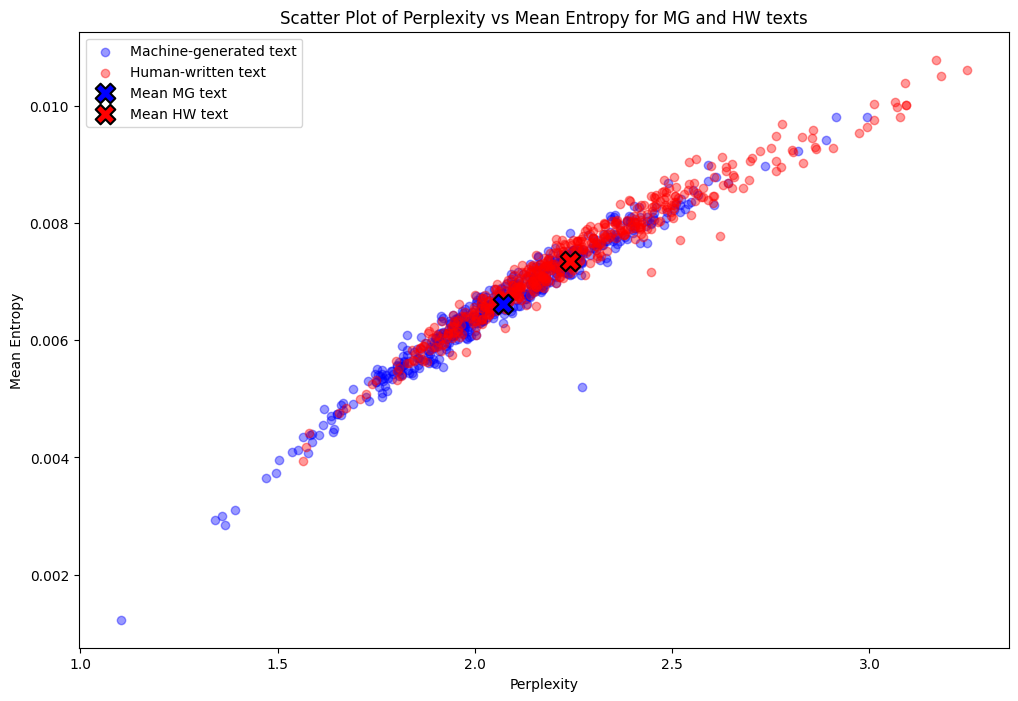
\includegraphics[width=\textwidth]{plot1.png}
	\caption{Perplexity distribution differs for different models.}
	\label{fig:schema}
\end{figure}

We processed texts from both labels using the LLM (Llama-3.1-8B-Instruct) and utilized contextual logits to compute two metrics: perplexity and entropy. By analyzing the distribution of points on the plane (Figure 1), a linear relationship between perplexity and entropy becomes evident. It is noticeable that the distribution of models is very different. Davinci and dolly have similar entropy as humans, while chatGPT and gpt4 is very different. This finding is promising, as it suggests that the distinction between MG and HW text distributions can potentially be detected using uncertainty estimation (UE). In the following sections, we explore this idea further to develop a more robust detection framework. 

\section{Conclusion}

\bibliographystyle{unsrtnat}
\bibliography{references.bib}

\end{document}